\section{Out of sample: a never-seen period}\label{sec:oos}

\para{Protocol:} The transfer rules were written to a file and hashed before any return on the new universe was computed (Appendix~\ref{app:prereg}). Only structural information was looked at beforehand: file layout, date range, rating counts, the cleaning log and signal coverage.
\begin{itemize}
  \item \emph{Frozen from development:} signals, LMH parameters, tranche period, allocator, costs and data rules
  \item \emph{Names per leg:} the development choice of 4 names out of 10 becomes a leg fraction of 0.4 of the names with a valid score each session, $k_t=\max(2,\lfloor 0.4N_t\rfloor)$ (primary). The literal $k=4$ is the secondary rule
  \item \emph{Evaluation window:} from 2024-01-05 to 2026-08-05 (647 sessions), after a 252-session warm-up
\end{itemize}
Nothing was changed afterwards.

\para{Results:} The primary book has a net Sharpe ratio of 1.05, a CAGR of 10.5\% at 10.0\% volatility, a maximum drawdown of $-8.0\%$ and a Calmar ratio of 1.32 (Table~\ref{tab:oos}, Figure~\ref{fig:oos}). Beta is $-0.02$ and the Jensen alpha 11.4\% a year ($t = 2.04$). The PSR is 0.95, and deflating over the two pre-registered variants leaves it at that level because the two are highly correlated. Both halves of the window are positive (Sharpe 1.44 and 0.88). The literal $k=4$ rule, four names per leg out of about 19, does worse (Sharpe 0.70, Calmar 0.72), in a wider universe breadth should grow with the universe, which is what the pre-registration says

\begin{table}[t]
\centering\footnotesize
\caption{Out of sample: frozen FMF-N over the never-seen period (net of 5\,bp)}\label{tab:oos}
\setlength{\tabcolsep}{4pt}
\begin{adjustbox}{max width=\textwidth}\begin{tabular}{lrrrrrrrrrrr}
\toprule
 & CAGR & Vol & Sharpe & MaxDD & Calmar & Beta & $\alpha$ & $t(\alpha)$ & PSR & Sharpe H1 & Sharpe H2\\
\midrule
FMF-N, primary (leg fraction 0.4) & 10.5 & 10.0 & 1.05 & $-8.0$ & 1.32 & $-0.02$ & 11.4 & 2.04 & 0.95 & 1.44 & 0.88\\
FMF-N, secondary ($k=4$) & 7.3 & 10.9 & 0.70 & $-10.2$ & 0.72 & $-0.04$ & 8.8 & 1.48 & 0.87 & 0.94 & 0.64\\
FMF-B20, beta budget 0.2 (exploratory)$^\dagger$ & 15.9 & 10.3 & 1.49 & $-6.5$ & 2.43 & 0.16 & 11.8 & 2.09 & 0.99 & 1.73 & 1.44\\
Equal-weight market (30 stocks) & 23.6 & 20.4 & 1.14 & $-25.3$ & 0.94 & 1.00 & -- & -- & 0.97 & 0.28 & 2.35\\
\bottomrule
\end{tabular}\end{adjustbox}
\par\smallskip\begin{minipage}{0.97\textwidth}\footnotesize Evaluation window 2024-01-05 to 2026-08-05. Percent per year for CAGR, volatility, drawdown and alpha. H1 and H2: halves of the window. $^\dagger$ Not in the pre-registration; the budget was fixed in development. Reported for information and used in no test.\end{minipage}
\end{table}

\para{The new signal replicates:} Out of sample LMH has an IC21 of 0.096 (one-sided $p = 0.042$), almost the development value (0.095; Table~\ref{tab:oos_signals}, Figure~\ref{fig:oos_ic}). Breadth (0.051) and the composite (0.073, $p = 0.065$) are positive. Event breadth is negative, but it covers only 26\% of stock-days: clusters of five same-day ratings are rare with 13 analysts per stock

\para{Against the toolkit, out of sample:} FMF-N is 2nd of 14 cross-sectional books on both Sharpe and Calmar (Table~\ref{tab:oos_league}, Figure~\ref{fig:oos_ic}). Only target-price momentum is ahead in this period (1.14 and 1.44). A 50/50 blend with FMF-N raises the Sharpe and Calmar ratios of all 16 comparables. The market and CTA-style trend have high Sharpe ratios in this bull period, with betas of 1.00 and 0.43 and drawdowns of $-25.3\%$ and $-10.8\%$

\para{Placebos and attribution:} The book beats IID random scores ($p = 0.027$) and is borderline against the stock-label permutation ($p = 0.056$). That figure comes from the notebook, whose permutations are unrestricted, so a few stocks keep their own signal in each draw; with derangements, as in development and in the package, $p = 0.046$. Against the circular time-shift it is not significant ($p = 0.226$), as in development (Table~\ref{tab:oos_placebo}). After the market and the four price-control books, alpha is 7.3\% ($t = 1.79$, $R^2 = 0.47$). With a 2.6-year window this is one more sample and not a proof. It is, however, the first sample never used for any choice, and both signatures of the method come back in it: zero beta with positive alpha, and LMH predicting returns

\begin{figure}[t]
\centering
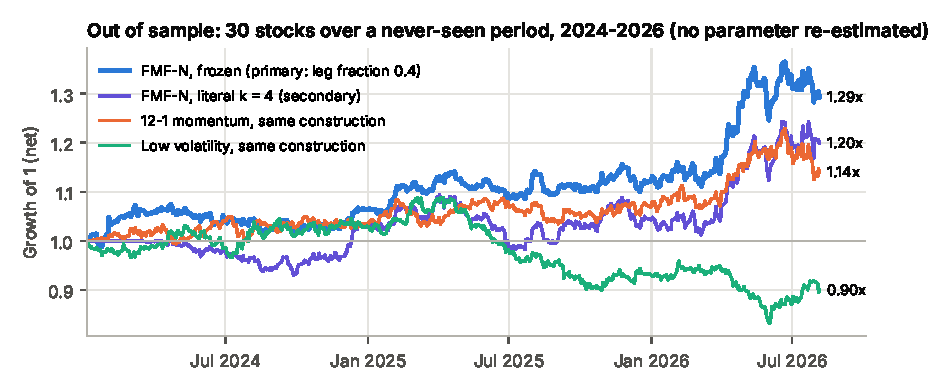
\includegraphics[width=\figw]{fig/fig11.pdf}
\caption{Growth of one unit over the never-seen period, frozen specification, net of 5\,bp.}\label{fig:oos}
\end{figure}

\begin{table}[t]
\centering\small
\caption{Out-of-sample signal evidence (labels inside the evaluation window)}\label{tab:oos_signals}
\begin{adjustbox}{max width=\textwidth}\begin{tabular}{lrrrrr}
\toprule
 & IC21 & $t_{\text{phase}}$ & $p$ & Hit (\%) & Coverage (\%)\\
\midrule
breadth\_63 & 0.051 & 0.98 & 0.168 & 58 & 47\\
event\_breadth\_63 & $-0.041$ & $-0.49$ & 0.685 & 46 & 26\\
breadth\_resid\_mom & 0.020 & 0.39 & 0.351 & 52 & 46\\
leader\_minus\_herd & 0.096 & 1.80 & 0.042 & 64 & 53\\
Composite & 0.073 & 1.56 & 0.065 & 58 & 59\\
\quad leaders only & 0.087 & 1.70 & 0.050 & 61 & 74\\
\bottomrule
\end{tabular}\end{adjustbox}
\end{table}

\begin{figure}[t]
\centering
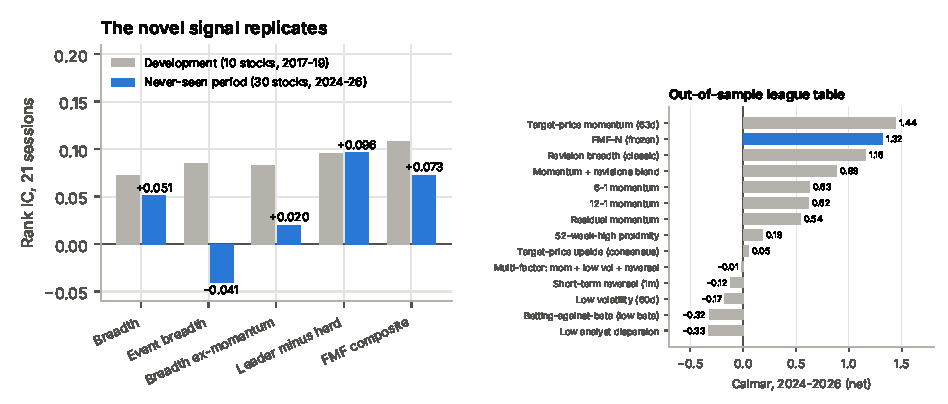
\includegraphics[width=\figw]{fig/fig12.pdf}
\caption{Left: rank IC (21 sessions) of each signal in development and over the never-seen period. Right: out-of-sample Calmar ratios of FMF-N and the cross-sectional comparables.}\label{fig:oos_ic}
\end{figure}

\begin{table}[t]
\centering\small
\caption{Out-of-sample placebo tests}\label{tab:oos_placebo}
\begin{adjustbox}{max width=\textwidth}\begin{tabular}{lrrrrr}
\toprule
Null & Draws & Sharpe & Null median & Null 95th & $p$\\
\midrule
IID random scores & 300 & 1.05 & $-0.26$ & 0.87 & 0.027\\
Stock-label permutation & 500 & 1.05 & $-0.01$ & 1.07 & 0.056\\
Circular time-shift & 216 & 1.05 & 0.09 & 2.17 & 0.226\\
\bottomrule
\end{tabular}\end{adjustbox}
\end{table}

\begin{table}[t]
\centering\footnotesize
\caption{Out of sample: FMF-N and institutional comparables}\label{tab:oos_league}
\begin{adjustbox}{max width=\textwidth}\begin{tabular}{lrrrrrrr}
\toprule
 & & & & & & \multicolumn{2}{c}{50/50 with FMF-N}\\
\cmidrule(lr){7-8}
 & Sharpe & Calmar & MaxDD (\%) & Beta & Corr.\ FMF-N & Sharpe & Calmar\\
\midrule
Time-series momentum 12-1 (CTA-style) & 1.30 & 1.62 & $-10.8$ & 0.43 & 0.33 & 1.45 & 1.86\\
Inverse-vol long-only (naive risk parity) & 1.23 & 1.01 & $-22.5$ & 0.88 & $-0.10$ & 1.66 & 1.56\\
Equal-weight long-only (market) & 1.14 & 0.94 & $-25.3$ & 1.00 & $-0.09$ & 1.54 & 1.41\\
Target-price momentum (63d) & 1.14 & 1.44 & $-7.5$ & 0.04 & 0.67 & 1.19 & 1.76\\
FMF-N (frozen) & 1.05 & 1.32 & $-8.0$ & $-0.02$ & 1.00 & -- & --\\
Revision breadth (classic) & 0.98 & 1.16 & $-8.7$ & $-0.01$ & 0.87 & 1.05 & 1.24\\
Momentum + revisions blend & 0.79 & 0.89 & $-8.2$ & 0.08 & 0.66 & 1.01 & 1.26\\
12-1 momentum (Jegadeesh-Titman) & 0.60 & 0.62 & $-8.5$ & 0.09 & 0.61 & 0.92 & 1.10\\
6-1 momentum & 0.56 & 0.63 & $-7.2$ & 0.04 & 0.63 & 0.91 & 1.09\\
Residual momentum (Blitz et al.) & 0.56 & 0.54 & $-7.9$ & 0.02 & 0.66 & 0.91 & 1.08\\
52-week-high proximity & 0.31 & 0.19 & $-12.0$ & $-0.09$ & 0.66 & 0.79 & 0.81\\
Target-price upside (consensus) & 0.11 & 0.05 & $-11.7$ & 0.05 & $-0.47$ & 1.19 & 1.50\\
Multi-factor: mom + low vol + reversal & 0.00 & $-0.01$ & $-14.3$ & $-0.13$ & 0.39 & 0.77 & 0.71\\
Short-term reversal (1m) & $-0.14$ & $-0.12$ & $-7.9$ & 0.00 & $-0.41$ & 1.05 & 1.07\\
Low volatility (60d) & $-0.39$ & $-0.17$ & $-23.5$ & $-0.26$ & 0.12 & 0.47 & 0.31\\
Low analyst dispersion & $-0.89$ & $-0.33$ & $-25.5$ & $-0.28$ & $-0.13$ & 0.17 & 0.10\\
Betting-against-beta (low beta) & $-0.94$ & $-0.32$ & $-34.3$ & $-0.33$ & $-0.19$ & $-0.04$ & $-0.04$\\
\bottomrule
\end{tabular}\end{adjustbox}
\end{table}

\para{Is the result carried by the ten development names?} Ten of the thirty names are the development stocks, seen again two years later. A post-hoc split, outside the pre-registration, re-runs the frozen specification on each part with the same GARCH forecasts. On the twenty names never used in development the book has a net Sharpe ratio of 0.80, a Calmar ratio of 0.98 and a maximum drawdown of $-9.2\%$, and LMH keeps its information coefficient (IC21 0.105, one-sided $p = 0.058$). The ten development names alone earn 0.31, with LMH near zero (0.022), but with sparse broker coverage a valid cross-section exists for only part of the window. The result is not a re-run of known names, and the new names, if anything, carry it. How the twenty names were chosen is another matter. They are today's large caps, a selection that already knows which companies grew large. A dollar-neutral book is exposed to this choice only through the spread between its legs, and the static tilt towards particular names loses money out of sample (Section~\ref{sec:identity})

\para{An exploratory check of the beta budget:} The pre-registration lists only the two market-neutral variants, so the beta-budget variant is reported apart and is used in no test. With the same scores and leg fraction and the budget $c=0.2$ fixed in development, FMF-B20 has a Sharpe ratio of 1.49, a Calmar ratio of 2.43 and a maximum drawdown of $-6.5\%$ at a beta of 0.16. The Jensen alpha does not change (11.8\% a year, $t = 2.09$), as expected, because the budget adds market return and no skill. In a bull window this is the expected direction. In a falling market the budget costs about $c$ times the market's loss, and for this reason it is a disclosed constant and not a timed bet
